\begin{figure*}[ht]

\tikzset{every picture/.style={line width=0.75pt}} %set default line width to 0.75pt        

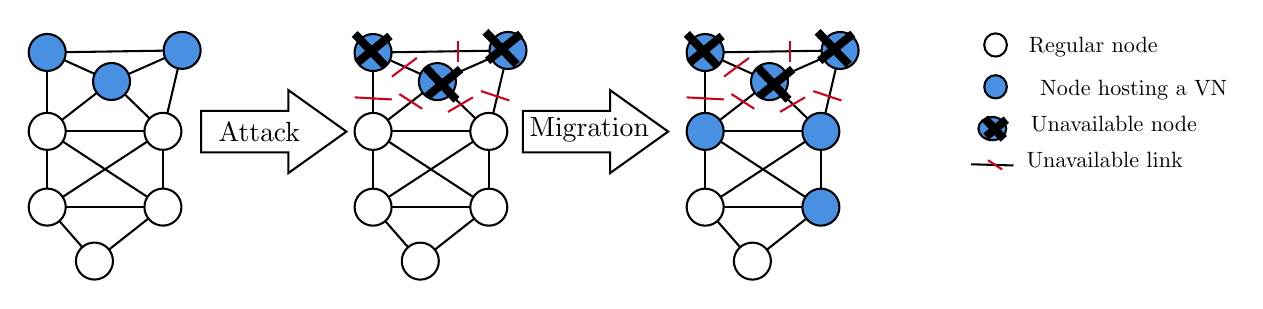
\begin{tikzpicture}[x=0.75pt,y=0.75pt,yscale=-1,xscale=1]
%uncomment if require: \path (0,300); %set diagram left start at 0, and has height of 300

%Shape: Ellipse [id:dp8430130954948494] 
\draw  [fill={rgb, 255:red, 74; green, 144; blue, 226 }  ,fill opacity=1 ] (461.48,51.56) .. controls (461.48,48.47) and (464.48,45.97) .. (468.19,45.97) .. controls (471.9,45.97) and (474.9,48.47) .. (474.9,51.56) .. controls (474.9,54.66) and (471.9,57.16) .. (468.19,57.16) .. controls (464.48,57.16) and (461.48,54.66) .. (461.48,51.56) -- cycle ;
%Shape: Ellipse [id:dp5907962461562573] 
\draw  [fill={rgb, 255:red, 74; green, 144; blue, 226 }  ,fill opacity=1 ] (464.29,31.43) .. controls (464.29,28.34) and (466.73,25.83) .. (469.74,25.83) .. controls (472.75,25.83) and (475.19,28.34) .. (475.19,31.43) .. controls (475.19,34.52) and (472.75,37.02) .. (469.74,37.02) .. controls (466.73,37.02) and (464.29,34.52) .. (464.29,31.43) -- cycle ;
%Straight Lines [id:da1514909222057811] 
\draw [color={rgb, 255:red, 0; green, 0; blue, 0 }  ,draw opacity=1 ]   (458,68.75) -- (478.38,69.32) ;


%Shape: Ellipse [id:dp8047559285598944] 
\draw  [fill={rgb, 255:red, 255; green, 255; blue, 255 }  ,fill opacity=1 ] (464.29,11.26) .. controls (464.29,8.17) and (466.73,5.67) .. (469.74,5.67) .. controls (472.75,5.67) and (475.19,8.17) .. (475.19,11.26) .. controls (475.19,14.35) and (472.75,16.86) .. (469.74,16.86) .. controls (466.73,16.86) and (464.29,14.35) .. (464.29,11.26) -- cycle ;
%Straight Lines [id:da5581047744563914] 
\draw [color={rgb, 255:red, 208; green, 2; blue, 27 }  ,draw opacity=1 ]   (472.87,71.26) -- (466.14,66.8) ;


%Straight Lines [id:da6983464143799673] 
\draw [line width=3]    (464.54,46.62) -- (473.71,56.51) ;


%Straight Lines [id:da20248481970311139] 
\draw [line width=3]    (465.15,55.41) -- (474.93,47.25) ;



%Straight Lines [id:da6176709448343998] 
\draw    (200.83,28.91) -- (225.58,52.91) ;


%Straight Lines [id:da5463688705908274] 
\draw    (200.83,28.91) -- (169.83,52.91) ;


%Straight Lines [id:da11538810799649779] 
\draw    (234.83,13.91) -- (225.92,51.91) ;


%Straight Lines [id:da8853756126147032] 
\draw    (169.83,14.91) -- (169.83,52.91) ;


%Straight Lines [id:da5031310157957251] 
\draw    (169.83,52.91) -- (225.58,89.41) ;


%Straight Lines [id:da8400043886929478] 
\draw    (169.83,89.41) -- (192.58,115.41) ;


%Straight Lines [id:da5242150334882041] 
\draw    (225.58,89.41) -- (192.58,115.41) ;


%Straight Lines [id:da3960630757961663] 
\draw    (225.58,52.91) -- (169.83,89.41) ;


%Shape: Circle [id:dp47175232960651714] 
\draw  [fill={rgb, 255:red, 255; green, 255; blue, 255 }  ,fill opacity=1 ] (160.92,52.91) .. controls (160.92,47.98) and (164.91,43.99) .. (169.83,43.99) .. controls (174.76,43.99) and (178.75,47.98) .. (178.75,52.91) .. controls (178.75,57.83) and (174.76,61.82) .. (169.83,61.82) .. controls (164.91,61.82) and (160.92,57.83) .. (160.92,52.91) -- cycle ;
%Shape: Circle [id:dp5879580381901867] 
\draw  [fill={rgb, 255:red, 255; green, 255; blue, 255 }  ,fill opacity=1 ] (216.67,52.91) .. controls (216.67,47.98) and (220.66,43.99) .. (225.58,43.99) .. controls (230.51,43.99) and (234.5,47.98) .. (234.5,52.91) .. controls (234.5,57.83) and (230.51,61.82) .. (225.58,61.82) .. controls (220.66,61.82) and (216.67,57.83) .. (216.67,52.91) -- cycle ;
%Shape: Circle [id:dp5579759383684684] 
\draw  [fill={rgb, 255:red, 255; green, 255; blue, 255 }  ,fill opacity=1 ] (160.92,89.41) .. controls (160.92,84.48) and (164.91,80.49) .. (169.83,80.49) .. controls (174.76,80.49) and (178.75,84.48) .. (178.75,89.41) .. controls (178.75,94.33) and (174.76,98.32) .. (169.83,98.32) .. controls (164.91,98.32) and (160.92,94.33) .. (160.92,89.41) -- cycle ;
%Shape: Circle [id:dp885869190555082] 
\draw  [fill={rgb, 255:red, 255; green, 255; blue, 255 }  ,fill opacity=1 ] (216.67,89.41) .. controls (216.67,84.48) and (220.66,80.49) .. (225.58,80.49) .. controls (230.51,80.49) and (234.5,84.48) .. (234.5,89.41) .. controls (234.5,94.33) and (230.51,98.32) .. (225.58,98.32) .. controls (220.66,98.32) and (216.67,94.33) .. (216.67,89.41) -- cycle ;
%Shape: Circle [id:dp3254884021888832] 
\draw  [fill={rgb, 255:red, 255; green, 255; blue, 255 }  ,fill opacity=1 ] (183.67,115.41) .. controls (183.67,110.48) and (187.66,106.49) .. (192.58,106.49) .. controls (197.51,106.49) and (201.5,110.48) .. (201.5,115.41) .. controls (201.5,120.33) and (197.51,124.32) .. (192.58,124.32) .. controls (187.66,124.32) and (183.67,120.33) .. (183.67,115.41) -- cycle ;
%Straight Lines [id:da7041582060743201] 
\draw    (178.75,52.91) -- (216.67,52.91) ;


%Straight Lines [id:da26176464493068274] 
\draw    (178.75,89.41) -- (216.67,89.41) ;


%Straight Lines [id:da45312150436944487] 
\draw    (225.58,80.49) -- (225.58,61.82) ;


%Straight Lines [id:da10497643854199257] 
\draw    (169.83,61.82) -- (169.83,80.49) ;


%Straight Lines [id:da023464273570334315] 
\draw    (169.83,14.91) -- (234.83,13.91) ;


%Straight Lines [id:da7461511731963238] 
\draw    (200.83,28.91) -- (234.83,13.91) ;


%Straight Lines [id:da6717008743630867] 
\draw    (169.83,14.91) -- (200.83,28.91) ;


%Shape: Circle [id:dp17672294199894456] 
\draw  [fill={rgb, 255:red, 74; green, 144; blue, 226 }  ,fill opacity=1 ] (160.92,14.91) .. controls (160.92,9.98) and (164.91,5.99) .. (169.83,5.99) .. controls (174.76,5.99) and (178.75,9.98) .. (178.75,14.91) .. controls (178.75,19.83) and (174.76,23.82) .. (169.83,23.82) .. controls (164.91,23.82) and (160.92,19.83) .. (160.92,14.91) -- cycle ;
%Shape: Circle [id:dp8878711028556632] 
\draw  [fill={rgb, 255:red, 74; green, 144; blue, 226 }  ,fill opacity=1 ] (191.92,28.91) .. controls (191.92,23.98) and (195.91,19.99) .. (200.83,19.99) .. controls (205.76,19.99) and (209.75,23.98) .. (209.75,28.91) .. controls (209.75,33.83) and (205.76,37.82) .. (200.83,37.82) .. controls (195.91,37.82) and (191.92,33.83) .. (191.92,28.91) -- cycle ;
%Shape: Circle [id:dp02560438280336974] 
\draw  [fill={rgb, 255:red, 74; green, 144; blue, 226 }  ,fill opacity=1 ] (225.92,13.91) .. controls (225.92,8.98) and (229.91,4.99) .. (234.83,4.99) .. controls (239.76,4.99) and (243.75,8.98) .. (243.75,13.91) .. controls (243.75,18.83) and (239.76,22.82) .. (234.83,22.82) .. controls (229.91,22.82) and (225.92,18.83) .. (225.92,13.91) -- cycle ;
%Straight Lines [id:da7816159630212767] 
\draw [color={rgb, 255:red, 208; green, 2; blue, 27 }  ,draw opacity=1 ]   (210.92,9.51) -- (210.92,19.51) ;


%Straight Lines [id:da23242280473047117] 
\draw [color={rgb, 255:red, 208; green, 2; blue, 27 }  ,draw opacity=1 ]   (221.92,33.51) -- (235.5,38.01) ;


%Straight Lines [id:da25217250177313655] 
\draw [color={rgb, 255:red, 208; green, 2; blue, 27 }  ,draw opacity=1 ]   (160.92,36.51) -- (178.92,37.51) ;


%Straight Lines [id:da8252457737222165] 
\draw [color={rgb, 255:red, 208; green, 2; blue, 27 }  ,draw opacity=1 ]   (178.92,26.51) -- (190.92,17.51) ;


%Straight Lines [id:da6307655523636441] 
\draw [color={rgb, 255:red, 208; green, 2; blue, 27 }  ,draw opacity=1 ]   (205.92,43.51) -- (217.92,36.51) ;


%Straight Lines [id:da5703265914230616] 
\draw [color={rgb, 255:red, 208; green, 2; blue, 27 }  ,draw opacity=1 ]   (193.5,42.01) -- (182.5,34.91) ;


%Straight Lines [id:da3989594608358942] 
\draw [line width=3]    (161,5.93) -- (176,21.68) ;


%Straight Lines [id:da7318288975856456] 
\draw [line width=3]    (162,19.93) -- (178,6.93) ;



%Straight Lines [id:da9963706937012238] 
\draw [line width=3]    (224,4.93) -- (239,20.68) ;


%Straight Lines [id:da43798340024618054] 
\draw [line width=3]    (225,18.93) -- (241,5.93) ;



%Straight Lines [id:da5033136183613764] 
\draw [line width=3]    (195,21.93) -- (210,37.68) ;


%Straight Lines [id:da623542865534238] 
\draw [line width=3]    (196,35.93) -- (212,22.93) ;




%Straight Lines [id:da021425369536150374] 
\draw    (43.83,28.87) -- (68.58,52.87) ;


%Straight Lines [id:da809644771756096] 
\draw    (43.83,28.87) -- (12.83,52.87) ;


%Straight Lines [id:da9075994171710501] 
\draw    (77.83,13.87) -- (68.92,51.87) ;


%Straight Lines [id:da7475460187374237] 
\draw    (12.83,14.87) -- (12.83,52.87) ;


%Straight Lines [id:da06975692875380135] 
\draw    (12.83,52.87) -- (68.58,89.37) ;


%Straight Lines [id:da9394544948671463] 
\draw    (12.83,89.37) -- (35.58,115.37) ;


%Straight Lines [id:da46361116523850066] 
\draw    (68.58,89.37) -- (35.58,115.37) ;


%Straight Lines [id:da9816638193583865] 
\draw    (68.58,52.87) -- (12.83,89.37) ;


%Shape: Circle [id:dp21531756732058427] 
\draw  [fill={rgb, 255:red, 255; green, 255; blue, 255 }  ,fill opacity=1 ] (3.92,52.87) .. controls (3.92,47.95) and (7.91,43.96) .. (12.83,43.96) .. controls (17.76,43.96) and (21.75,47.95) .. (21.75,52.87) .. controls (21.75,57.8) and (17.76,61.79) .. (12.83,61.79) .. controls (7.91,61.79) and (3.92,57.8) .. (3.92,52.87) -- cycle ;
%Shape: Circle [id:dp32258921480580105] 
\draw  [fill={rgb, 255:red, 255; green, 255; blue, 255 }  ,fill opacity=1 ] (59.67,52.87) .. controls (59.67,47.95) and (63.66,43.96) .. (68.58,43.96) .. controls (73.51,43.96) and (77.5,47.95) .. (77.5,52.87) .. controls (77.5,57.8) and (73.51,61.79) .. (68.58,61.79) .. controls (63.66,61.79) and (59.67,57.8) .. (59.67,52.87) -- cycle ;
%Shape: Circle [id:dp7783815840311967] 
\draw  [fill={rgb, 255:red, 255; green, 255; blue, 255 }  ,fill opacity=1 ] (3.92,89.37) .. controls (3.92,84.45) and (7.91,80.46) .. (12.83,80.46) .. controls (17.76,80.46) and (21.75,84.45) .. (21.75,89.37) .. controls (21.75,94.3) and (17.76,98.29) .. (12.83,98.29) .. controls (7.91,98.29) and (3.92,94.3) .. (3.92,89.37) -- cycle ;
%Shape: Circle [id:dp9106798970146953] 
\draw  [fill={rgb, 255:red, 255; green, 255; blue, 255 }  ,fill opacity=1 ] (59.67,89.37) .. controls (59.67,84.45) and (63.66,80.46) .. (68.58,80.46) .. controls (73.51,80.46) and (77.5,84.45) .. (77.5,89.37) .. controls (77.5,94.3) and (73.51,98.29) .. (68.58,98.29) .. controls (63.66,98.29) and (59.67,94.3) .. (59.67,89.37) -- cycle ;
%Shape: Circle [id:dp1831427544072476] 
\draw  [fill={rgb, 255:red, 255; green, 255; blue, 255 }  ,fill opacity=1 ] (26.67,115.37) .. controls (26.67,110.45) and (30.66,106.46) .. (35.58,106.46) .. controls (40.51,106.46) and (44.5,110.45) .. (44.5,115.37) .. controls (44.5,120.3) and (40.51,124.29) .. (35.58,124.29) .. controls (30.66,124.29) and (26.67,120.3) .. (26.67,115.37) -- cycle ;
%Straight Lines [id:da9700158448121917] 
\draw    (21.75,52.87) -- (59.67,52.87) ;


%Straight Lines [id:da010185511635833033] 
\draw    (21.75,89.37) -- (59.67,89.37) ;


%Straight Lines [id:da4677014236726348] 
\draw    (68.58,80.46) -- (68.58,61.79) ;


%Straight Lines [id:da19862578341507608] 
\draw    (12.83,61.79) -- (12.83,80.46) ;


%Straight Lines [id:da6877311034443738] 
\draw    (12.83,14.87) -- (77.83,13.87) ;


%Straight Lines [id:da39601253001890035] 
\draw    (43.83,28.87) -- (77.83,13.87) ;


%Straight Lines [id:da8270994037474519] 
\draw    (12.83,14.87) -- (43.83,28.87) ;


%Shape: Circle [id:dp2984826737185816] 
\draw  [fill={rgb, 255:red, 74; green, 144; blue, 226 }  ,fill opacity=1 ] (3.92,14.87) .. controls (3.92,9.95) and (7.91,5.96) .. (12.83,5.96) .. controls (17.76,5.96) and (21.75,9.95) .. (21.75,14.87) .. controls (21.75,19.8) and (17.76,23.79) .. (12.83,23.79) .. controls (7.91,23.79) and (3.92,19.8) .. (3.92,14.87) -- cycle ;
%Shape: Circle [id:dp6437572475375565] 
\draw  [fill={rgb, 255:red, 74; green, 144; blue, 226 }  ,fill opacity=1 ] (34.92,28.87) .. controls (34.92,23.95) and (38.91,19.96) .. (43.83,19.96) .. controls (48.76,19.96) and (52.75,23.95) .. (52.75,28.87) .. controls (52.75,33.8) and (48.76,37.79) .. (43.83,37.79) .. controls (38.91,37.79) and (34.92,33.8) .. (34.92,28.87) -- cycle ;
%Shape: Circle [id:dp23183818676236623] 
\draw  [fill={rgb, 255:red, 74; green, 144; blue, 226 }  ,fill opacity=1 ] (68.92,13.87) .. controls (68.92,8.95) and (72.91,4.96) .. (77.83,4.96) .. controls (82.76,4.96) and (86.75,8.95) .. (86.75,13.87) .. controls (86.75,18.8) and (82.76,22.79) .. (77.83,22.79) .. controls (72.91,22.79) and (68.92,18.8) .. (68.92,13.87) -- cycle ;

%Right Arrow [id:dp417684980473099] 
\draw   (87,43) -- (129,43) -- (129,33) -- (157,53) -- (129,73) -- (129,63) -- (87,63) -- cycle ;

%Right Arrow [id:dp6623970589974628] 
\draw   (242,43) -- (284,43) -- (284,33) -- (312,53) -- (284,73) -- (284,63) -- (242,63) -- cycle ;
%Straight Lines [id:da22163993557127015] 
\draw    (360.83,28.91) -- (385.58,52.91) ;


%Straight Lines [id:da8341652491193966] 
\draw    (360.83,28.91) -- (329.83,52.91) ;


%Straight Lines [id:da14662408338887967] 
\draw    (394.83,13.91) -- (385.92,51.91) ;


%Straight Lines [id:da1054361182628697] 
\draw    (329.83,14.91) -- (329.83,52.91) ;


%Straight Lines [id:da878058282787745] 
\draw    (329.83,52.91) -- (385.58,89.41) ;


%Straight Lines [id:da5143639640863213] 
\draw    (329.83,89.41) -- (352.58,115.41) ;


%Straight Lines [id:da38106162801473] 
\draw    (385.58,89.41) -- (352.58,115.41) ;


%Straight Lines [id:da9515281954413589] 
\draw    (385.58,52.91) -- (329.83,89.41) ;


%Shape: Circle [id:dp7012949201072771] 
\draw  [fill={rgb, 255:red, 74; green, 144; blue, 226 }  ,fill opacity=1 ] (320.92,52.91) .. controls (320.92,47.98) and (324.91,43.99) .. (329.83,43.99) .. controls (334.76,43.99) and (338.75,47.98) .. (338.75,52.91) .. controls (338.75,57.83) and (334.76,61.82) .. (329.83,61.82) .. controls (324.91,61.82) and (320.92,57.83) .. (320.92,52.91) -- cycle ;
%Shape: Circle [id:dp8511635916765001] 
\draw  [fill={rgb, 255:red, 74; green, 144; blue, 226 }  ,fill opacity=1 ] (376.67,52.91) .. controls (376.67,47.98) and (380.66,43.99) .. (385.58,43.99) .. controls (390.51,43.99) and (394.5,47.98) .. (394.5,52.91) .. controls (394.5,57.83) and (390.51,61.82) .. (385.58,61.82) .. controls (380.66,61.82) and (376.67,57.83) .. (376.67,52.91) -- cycle ;
%Shape: Circle [id:dp10253503783482376] 
\draw  [fill={rgb, 255:red, 255; green, 255; blue, 255 }  ,fill opacity=1 ] (320.92,89.41) .. controls (320.92,84.48) and (324.91,80.49) .. (329.83,80.49) .. controls (334.76,80.49) and (338.75,84.48) .. (338.75,89.41) .. controls (338.75,94.33) and (334.76,98.32) .. (329.83,98.32) .. controls (324.91,98.32) and (320.92,94.33) .. (320.92,89.41) -- cycle ;
%Shape: Circle [id:dp7321236156986349] 
\draw  [fill={rgb, 255:red, 74; green, 144; blue, 226 }  ,fill opacity=1 ] (376.67,89.41) .. controls (376.67,84.48) and (380.66,80.49) .. (385.58,80.49) .. controls (390.51,80.49) and (394.5,84.48) .. (394.5,89.41) .. controls (394.5,94.33) and (390.51,98.32) .. (385.58,98.32) .. controls (380.66,98.32) and (376.67,94.33) .. (376.67,89.41) -- cycle ;
%Shape: Circle [id:dp8317705860942972] 
\draw  [fill={rgb, 255:red, 255; green, 255; blue, 255 }  ,fill opacity=1 ] (343.67,115.41) .. controls (343.67,110.48) and (347.66,106.49) .. (352.58,106.49) .. controls (357.51,106.49) and (361.5,110.48) .. (361.5,115.41) .. controls (361.5,120.33) and (357.51,124.32) .. (352.58,124.32) .. controls (347.66,124.32) and (343.67,120.33) .. (343.67,115.41) -- cycle ;
%Straight Lines [id:da11492821108610518] 
\draw    (338.75,52.91) -- (376.67,52.91) ;


%Straight Lines [id:da6428199077173957] 
\draw    (338.75,89.41) -- (376.67,89.41) ;


%Straight Lines [id:da4443653918115038] 
\draw    (385.58,80.49) -- (385.58,61.82) ;


%Straight Lines [id:da5181998888947625] 
\draw    (329.83,61.82) -- (329.83,80.49) ;


%Straight Lines [id:da8991729748789462] 
\draw    (329.83,14.91) -- (394.83,13.91) ;


%Straight Lines [id:da6133921287796495] 
\draw    (360.83,28.91) -- (394.83,13.91) ;


%Straight Lines [id:da3198353622868253] 
\draw    (329.83,14.91) -- (360.83,28.91) ;


%Shape: Circle [id:dp32555515723538997] 
\draw  [fill={rgb, 255:red, 74; green, 144; blue, 226 }  ,fill opacity=1 ] (320.92,14.91) .. controls (320.92,9.98) and (324.91,5.99) .. (329.83,5.99) .. controls (334.76,5.99) and (338.75,9.98) .. (338.75,14.91) .. controls (338.75,19.83) and (334.76,23.82) .. (329.83,23.82) .. controls (324.91,23.82) and (320.92,19.83) .. (320.92,14.91) -- cycle ;
%Shape: Circle [id:dp479820223624436] 
\draw  [fill={rgb, 255:red, 74; green, 144; blue, 226 }  ,fill opacity=1 ] (351.92,28.91) .. controls (351.92,23.98) and (355.91,19.99) .. (360.83,19.99) .. controls (365.76,19.99) and (369.75,23.98) .. (369.75,28.91) .. controls (369.75,33.83) and (365.76,37.82) .. (360.83,37.82) .. controls (355.91,37.82) and (351.92,33.83) .. (351.92,28.91) -- cycle ;
%Shape: Circle [id:dp49048798397317805] 
\draw  [fill={rgb, 255:red, 74; green, 144; blue, 226 }  ,fill opacity=1 ] (385.92,13.91) .. controls (385.92,8.98) and (389.91,4.99) .. (394.83,4.99) .. controls (399.76,4.99) and (403.75,8.98) .. (403.75,13.91) .. controls (403.75,18.83) and (399.76,22.82) .. (394.83,22.82) .. controls (389.91,22.82) and (385.92,18.83) .. (385.92,13.91) -- cycle ;
%Straight Lines [id:da2877242408536883] 
\draw [color={rgb, 255:red, 208; green, 2; blue, 27 }  ,draw opacity=1 ]   (370.92,9.51) -- (370.92,19.51) ;


%Straight Lines [id:da384891491483089] 
\draw [color={rgb, 255:red, 208; green, 2; blue, 27 }  ,draw opacity=1 ]   (381.92,33.51) -- (395.5,38.01) ;


%Straight Lines [id:da9676951250293255] 
\draw [color={rgb, 255:red, 208; green, 2; blue, 27 }  ,draw opacity=1 ]   (320.92,36.51) -- (338.92,37.51) ;


%Straight Lines [id:da8030081016605746] 
\draw [color={rgb, 255:red, 208; green, 2; blue, 27 }  ,draw opacity=1 ]   (338.92,26.51) -- (350.92,17.51) ;


%Straight Lines [id:da14577170595095879] 
\draw [color={rgb, 255:red, 208; green, 2; blue, 27 }  ,draw opacity=1 ]   (365.92,43.51) -- (377.92,36.51) ;


%Straight Lines [id:da1498283509390178] 
\draw [color={rgb, 255:red, 208; green, 2; blue, 27 }  ,draw opacity=1 ]   (353.5,42.01) -- (342.5,34.91) ;


%Straight Lines [id:da7540175814554593] 
\draw [line width=3]    (321,5.93) -- (336,21.68) ;


%Straight Lines [id:da08956624030773497] 
\draw [line width=3]    (322,19.93) -- (338,6.93) ;



%Straight Lines [id:da4115477309546427] 
\draw [line width=3]    (384,4.93) -- (399,20.68) ;


%Straight Lines [id:da6038706591283135] 
\draw [line width=3]    (385,18.93) -- (401,5.93) ;



%Straight Lines [id:da5077658828074341] 
\draw [line width=3]    (355,21.93) -- (370,37.68) ;


%Straight Lines [id:da9268834839804526] 
\draw [line width=3]    (356,35.93) -- (372,22.93) ;




% Text Node
\draw (516.81,12.09) node [scale=0.8] [align=left] {Regular node};
% Text Node
\draw (536.31,33.08) node [scale=0.8] [align=left] {Node hosting a VN};
% Text Node
\draw (526.81,49.09) node [scale=0.8] [align=left] {Unavailable node};
% Text Node
\draw (522.31,66.56) node [scale=0.8] [align=left] {Unavailable link};
% Text Node
\draw (274,52) node  [align=left] {Migration};
% Text Node
\draw (115,53) node  [align=left] {Attack};


\end{tikzpicture}



\caption{Migration triggered by the attacker}
\label{fig:trigger}

\end{figure*}

\subsubsection{Attacker model}
\label{sec:attack_model}
Fig.~\ref{fig:trigger} depicts the evolution of the infrastructure once the attacker makes part of it unavailable. 
At first, the virtual network is running on a healthy physical substrate; but once the attack is launched, the substrate becomes unavailable and the virtual network must be migrated quickly to reduce the end user's service interruption.
The success of the attacks on the migration relies on two main aspects: the ability to affect the configuration of SDN nodes as well as  to retrieve the exfiltrated data.
While the latter can be easily solved by owning virtual machines in the infrastructure, the former requires to be able to alter nodes configuration. This has been proven possible in~\cite{Taxonomy_Hizver2015, Bokani2015, attain-Ujcich2017}.
Precisely, the attacker is able to spoof the identity of the network hypervisor, and thus is able to inject malicious flow rules inside the nodes to create the data exfiltration path. 
However, he is not able to be designated as the original network hypervisor in the nodes' configurations. 
% \GB{not completely clear}\FC{Better ?}. 
This can be explained because it requires advanced configuration privileges. Moreover, a physical node missing from the legitimate hypervisor's topology view is easily detectable, in comparison to malicious flow rules injected inside the physical nodes.
% \FC{If keeping this part we will need an introduction to SDN, probably will need one anyway}\FC{This can be explained because it requires advanced configuration privileges, and moreover, a physical node missing is easily detectable by the legitimate controller compared to a misconfiguration on a swi/attacking switch, not proxifying the communication}
Even though the virtualization infrastructure hosts several virtual networks and end users, we limit the scope of the attacker to a unique target virtual network. 
% The attacker is motivated to attack a particular user inside the infrastructure, thus targeting one particular virtual network. 
He has been able to determine which nodes to attack to trigger the migration thanks to prior scanning and information gathering. 
% ~\GB{you mean ``reconnaissance'' and ``scanning''}
Nevertheless, he has no exact knowledge about which nodes will be selected as the destination substrate and he will discover it by doing further scanning and fingerprinting  while he is attacking the infrastructure.  
Even if the attacker may target all nodes in the infrastructure, he has no incentives to attack nodes that will not contribute to exfiltrate data from his victim's network. 
% \GB{so to identify them, the attacker has to have some global visibility, which she gets from scanning. Is it feasible?}

% \GB{you already said that earlier. Can you be more specific now?}\FC{Aren't the provided sources enough ?}
We can find a description of such techniques in~\cite{Hong2015,Sphinx-Dhawan2015}.
This information gathering is not depicted in this paper and we consider that the attacker will choose his targets as presented in Section~\ref{sec:target_proba}.
From the point of view of the defender, it is impossible to accurately know which node will be attacked.
% in the infrastructure.
% \GB{of the future substrate? or any physical node from the infrastructure?}.
The attacker may own several virtual machines inside the infrastructure, thus has several sources to launch an attack. However, he can only attack one node at a time. 
We suppose that each node will always be attacked from the same source. 
Because of the short time interval considered for the migration, we suppose that the attack will always take the same path. 
This path will be considered to determine the global detection probability of the attack.
% , since all the nodes monitoring the path may see the attack come through.
% \GB{so this is very important to understand at what level is located the attacker. Is she another tenant? Or does she have access to the substrate? Do attack packets flow at the data plane or at the control plane?}.\FC{The attack is routed in the control plane but impacts the data plane. I don't want to go to deep in details so we do not add too much confusion. We can simplify by saying that the control plane topology is the same as the data plane topology.}


\begin{figure*}[htbp]


\tikzset{every picture/.style={line width=0.75pt}} %set default line width to 0.75pt        

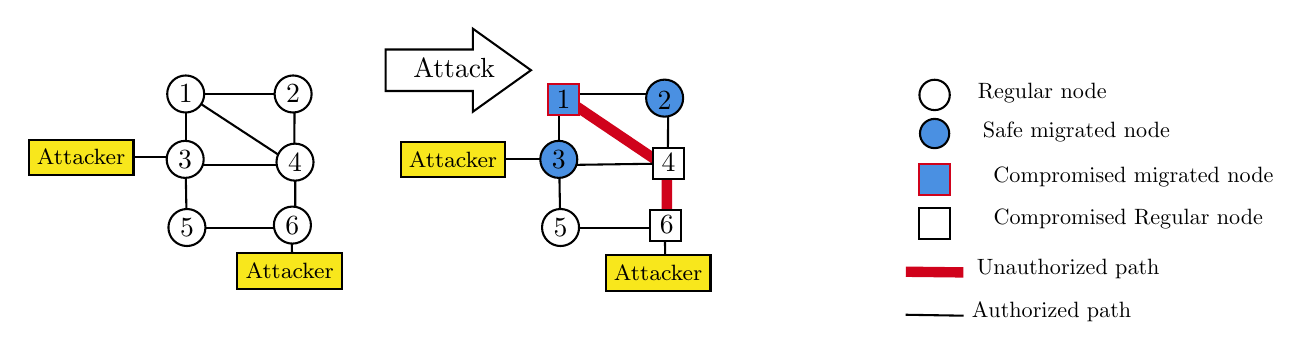
\begin{tikzpicture}[x=0.75pt,y=0.75pt,yscale=-1,xscale=1]
%uncomment if require: \path (0,300); %set diagram left start at 0, and has height of 300

%Straight Lines [id:da7739123357617682] 
\draw    (70.75,83.4) -- (108.67,83.4) ;


%Shape: Rectangle [id:dp46476407013383825] 
\draw  [fill={rgb, 255:red, 248; green, 231; blue, 28 }  ,fill opacity=1 ] (29.2,75.2) -- (79.67,75.2) -- (79.67,92.18) -- (29.2,92.18) -- cycle ;


%Straight Lines [id:da13064923443841459] 
\draw    (249.95,84.6) -- (287.87,84.6) ;


%Shape: Rectangle [id:dp28554238318371994] 
\draw  [fill={rgb, 255:red, 248; green, 231; blue, 28 }  ,fill opacity=1 ] (208.4,76.4) -- (258.87,76.4) -- (258.87,93.38) -- (208.4,93.38) -- cycle ;


%Straight Lines [id:da567285896843154] 
\draw [color={rgb, 255:red, 208; green, 2; blue, 27 }  ,draw opacity=1 ][line width=3.75]    (336.65,85.21) -- (336.67,119) ;


%Straight Lines [id:da046576842172091903] 
\draw [color={rgb, 255:red, 208; green, 2; blue, 27 }  ,draw opacity=1 ][line width=3.75]    (290.52,57.47) -- (333.33,86.33) ;


%Straight Lines [id:da5668243278416182] 
\draw    (157.33,49.22) -- (157.17,80.81) ;


%Straight Lines [id:da49434419911731065] 
\draw    (111.08,117.73) -- (149,117.73) ;


%Straight Lines [id:da6673139716829495] 
\draw    (155.58,114.06) -- (156.5,144) ;


%Straight Lines [id:da9840681038768349] 
\draw    (104.83,53.23) -- (160.58,89.73) ;


%Straight Lines [id:da4482722852442499] 
\draw    (104.83,89.73) -- (105.33,117.55) ;


%Straight Lines [id:da7670268694366985] 
\draw    (157.58,87.73) -- (157.67,119.88) ;


%Shape: Circle [id:dp667695613861877] 
\draw  [fill={rgb, 255:red, 255; green, 255; blue, 255 }  ,fill opacity=1 ] (95.92,53.23) .. controls (95.92,48.3) and (99.91,44.31) .. (104.83,44.31) .. controls (109.76,44.31) and (113.75,48.3) .. (113.75,53.23) .. controls (113.75,58.15) and (109.76,62.15) .. (104.83,62.15) .. controls (99.91,62.15) and (95.92,58.15) .. (95.92,53.23) -- cycle ;

%Shape: Circle [id:dp7262621996740888] 
\draw  [fill={rgb, 255:red, 255; green, 255; blue, 255 }  ,fill opacity=1 ] (148.58,86.06) .. controls (148.58,81.14) and (152.58,77.15) .. (157.5,77.15) .. controls (162.42,77.15) and (166.42,81.14) .. (166.42,86.06) .. controls (166.42,90.99) and (162.42,94.98) .. (157.5,94.98) .. controls (152.58,94.98) and (148.58,90.99) .. (148.58,86.06) -- cycle ;

%Shape: Circle [id:dp08856327459465119] 
\draw  [fill={rgb, 255:red, 255; green, 255; blue, 255 }  ,fill opacity=1 ] (147.33,116.4) .. controls (147.33,111.47) and (151.33,107.48) .. (156.25,107.48) .. controls (161.17,107.48) and (165.17,111.47) .. (165.17,116.4) .. controls (165.17,121.32) and (161.17,125.31) .. (156.25,125.31) .. controls (151.33,125.31) and (147.33,121.32) .. (147.33,116.4) -- cycle ;

%Straight Lines [id:da658208744911517] 
\draw    (113.75,53.23) -- (151.67,53.23) ;


%Straight Lines [id:da49379806707152474] 
\draw    (110.75,87.4) -- (148.67,87.4) ;


%Straight Lines [id:da6945831753833721] 
\draw    (104.83,62.15) -- (104.83,80.81) ;


%Shape: Circle [id:dp7034065447291917] 
\draw  [fill={rgb, 255:red, 255; green, 255; blue, 255 }  ,fill opacity=1 ] (96.52,117.56) .. controls (96.52,112.64) and (100.51,108.65) .. (105.43,108.65) .. controls (110.36,108.65) and (114.35,112.64) .. (114.35,117.56) .. controls (114.35,122.49) and (110.36,126.48) .. (105.43,126.48) .. controls (100.51,126.48) and (96.52,122.49) .. (96.52,117.56) -- cycle ;

%Shape: Circle [id:dp4778597289311547] 
\draw  [fill={rgb, 255:red, 255; green, 255; blue, 255 }  ,fill opacity=1 ] (95.67,84.73) .. controls (95.67,79.8) and (99.66,75.81) .. (104.58,75.81) .. controls (109.51,75.81) and (113.5,79.8) .. (113.5,84.73) .. controls (113.5,89.65) and (109.51,93.65) .. (104.58,93.65) .. controls (99.66,93.65) and (95.67,89.65) .. (95.67,84.73) -- cycle ;

%Shape: Circle [id:dp08437409893269954] 
\draw  [fill={rgb, 255:red, 255; green, 255; blue, 255 }  ,fill opacity=1 ] (147.67,53.23) .. controls (147.67,48.3) and (151.66,44.31) .. (156.58,44.31) .. controls (161.51,44.31) and (165.5,48.3) .. (165.5,53.23) .. controls (165.5,58.15) and (161.51,62.15) .. (156.58,62.15) .. controls (151.66,62.15) and (147.67,58.15) .. (147.67,53.23) -- cycle ;

%Shape: Circle [id:dp2544455966731902] 
\draw  [fill={rgb, 255:red, 74; green, 144; blue, 226 }  ,fill opacity=1 ] (458.61,72.28) .. controls (458.61,68.39) and (461.76,65.23) .. (465.66,65.23) .. controls (469.55,65.23) and (472.71,68.39) .. (472.71,72.28) .. controls (472.71,76.18) and (469.55,79.33) .. (465.66,79.33) .. controls (461.76,79.33) and (458.61,76.18) .. (458.61,72.28) -- cycle ;
%Straight Lines [id:da3025029961647492] 
\draw [color={rgb, 255:red, 208; green, 2; blue, 27 }  ,draw opacity=1 ][line width=3.75]    (451.78,138.87) -- (479.53,139.19) ;


%Shape: Circle [id:dp2181751678296382] 
\draw  [fill={rgb, 255:red, 255; green, 255; blue, 255 }  ,fill opacity=1 ] (458.35,53.69) .. controls (458.35,49.65) and (461.62,46.37) .. (465.66,46.37) .. controls (469.7,46.37) and (472.97,49.65) .. (472.97,53.69) .. controls (472.97,57.73) and (469.7,61) .. (465.66,61) .. controls (461.62,61) and (458.35,57.73) .. (458.35,53.69) -- cycle ;
%Straight Lines [id:da9324723367639798] 
\draw [color={rgb, 255:red, 0; green, 0; blue, 0 }  ,draw opacity=1 ]   (451.64,159.59) -- (479.68,160.05) ;


%Shape: Square [id:dp642864286437786] 
\draw  [color={rgb, 255:red, 208; green, 2; blue, 27 }  ,draw opacity=1 ][fill={rgb, 255:red, 74; green, 144; blue, 226 }  ,fill opacity=1 ] (458.16,86.93) -- (473.16,86.93) -- (473.16,101.93) -- (458.16,101.93) -- cycle ;
%Shape: Square [id:dp6103038230457687] 
\draw  [fill={rgb, 255:red, 255; green, 255; blue, 255 }  ,fill opacity=1 ] (458.16,108.16) -- (473.16,108.16) -- (473.16,123.16) -- (458.16,123.16) -- cycle ;

%Right Arrow [id:dp9004425172478334] 
\draw  [fill={rgb, 255:red, 255; green, 255; blue, 255 }  ,fill opacity=1 ] (201.2,31.78) -- (243.2,31.78) -- (243.2,21.78) -- (271.2,41.78) -- (243.2,61.78) -- (243.2,51.78) -- (201.2,51.78) -- cycle ;

%Straight Lines [id:da8396173497547912] 
\draw    (337.33,49.22) -- (337.17,80.81) ;


%Straight Lines [id:da9182383261146002] 
\draw    (291.08,117.73) -- (329,117.73) ;


%Straight Lines [id:da858414453735221] 
\draw    (335.58,114.06) -- (336,140.5) ;


%Straight Lines [id:da20295515063433045] 
\draw    (284.83,89.73) -- (285.33,117.55) ;


%Straight Lines [id:da24824224288757746] 
\draw    (293.75,53.23) -- (331.67,53.23) ;


%Straight Lines [id:da32113645413312253] 
\draw    (290.75,87.4) -- (337.58,86.73) ;


%Straight Lines [id:da20280015358357328] 
\draw    (284.83,62.15) -- (284.83,80.81) ;


%Shape: Circle [id:dp2078999158258219] 
\draw  [fill={rgb, 255:red, 255; green, 255; blue, 255 }  ,fill opacity=1 ] (276.52,117.56) .. controls (276.52,112.64) and (280.51,108.65) .. (285.43,108.65) .. controls (290.36,108.65) and (294.35,112.64) .. (294.35,117.56) .. controls (294.35,122.49) and (290.36,126.48) .. (285.43,126.48) .. controls (280.51,126.48) and (276.52,122.49) .. (276.52,117.56) -- cycle ;

%Shape: Circle [id:dp17283437144421832] 
\draw  [fill={rgb, 255:red, 74; green, 144; blue, 226 }  ,fill opacity=1 ] (275.67,84.73) .. controls (275.67,79.8) and (279.66,75.81) .. (284.58,75.81) .. controls (289.51,75.81) and (293.5,79.8) .. (293.5,84.73) .. controls (293.5,89.65) and (289.51,93.65) .. (284.58,93.65) .. controls (279.66,93.65) and (275.67,89.65) .. (275.67,84.73) -- cycle ;

%Shape: Circle [id:dp6292985525556183] 
\draw  [fill={rgb, 255:red, 74; green, 144; blue, 226 }  ,fill opacity=1 ] (326.67,55.23) .. controls (326.67,50.3) and (330.66,46.31) .. (335.58,46.31) .. controls (340.51,46.31) and (344.5,50.3) .. (344.5,55.23) .. controls (344.5,60.15) and (340.51,64.15) .. (335.58,64.15) .. controls (330.66,64.15) and (326.67,60.15) .. (326.67,55.23) -- cycle ;

%Shape: Square [id:dp21738038837827933] 
\draw  [color={rgb, 255:red, 208; green, 2; blue, 27 }  ,draw opacity=1 ][fill={rgb, 255:red, 74; green, 144; blue, 226 }  ,fill opacity=1 ] (279.37,48.2) -- (294.37,48.2) -- (294.37,63.2) -- (279.37,63.2) -- cycle ;
%Shape: Square [id:dp8476679341444072] 
\draw  [fill={rgb, 255:red, 255; green, 255; blue, 255 }  ,fill opacity=1 ] (330.08,79.23) -- (345.08,79.23) -- (345.08,94.23) -- (330.08,94.23) -- cycle ;

%Shape: Square [id:dp8795975156412624] 
\draw  [fill={rgb, 255:red, 255; green, 255; blue, 255 }  ,fill opacity=1 ] (328.48,109.23) -- (343.48,109.23) -- (343.48,124.23) -- (328.48,124.23) -- cycle ;
%Shape: Rectangle [id:dp2088885864598815] 
\draw  [fill={rgb, 255:red, 248; green, 231; blue, 28 }  ,fill opacity=1 ] (129.7,130) -- (180.17,130) -- (180.17,146.98) -- (129.7,146.98) -- cycle ;

%Shape: Rectangle [id:dp5309747919784684] 
\draw  [fill={rgb, 255:red, 248; green, 231; blue, 28 }  ,fill opacity=1 ] (307.2,131) -- (357.67,131) -- (357.67,147.98) -- (307.2,147.98) -- cycle ;


% Text Node
\draw (336.65,116) node  [align=left] {6};
% Text Node
\draw (286.87,55.7) node  [align=left] {1};
% Text Node
\draw (332.44,139.49) node  [align=left] {{\footnotesize Attacker}};
% Text Node
\draw (154.94,138.49) node  [align=left] {{\footnotesize Attacker}};
% Text Node
\draw (337.5,86.06) node  [align=left] {4};
% Text Node
\draw (335.58,56.23) node  [align=left] {2};
% Text Node
\draw (284.58,84.73) node  [align=left] {3};
% Text Node
\draw (285.43,117.56) node  [align=left] {5};
% Text Node
\draw (234.2,40.8) node  [align=left] {Attack};
% Text Node
\draw (522,158.05) node [scale=0.8] [align=left] {Authorized path};
% Text Node
\draw (530,137.33) node [scale=0.8] [align=left] {Unauthorized path};
% Text Node
\draw (559,113.58) node [scale=0.8] [align=left] {Compromised Regular node};
% Text Node
\draw (561.5,93.17) node [scale=0.8] [align=left] {Compromised migrated node};
% Text Node
\draw (534,71.48) node [scale=0.8] [align=left] {Safe migrated node};
% Text Node
\draw (517.5,52.62) node [scale=0.8] [align=left] {Regular node};
% Text Node
\draw (156.58,53.23) node  [align=left] {2};
% Text Node
\draw (104.58,84.73) node  [align=left] {3};
% Text Node
\draw (105.43,117.56) node  [align=left] {5};
% Text Node
\draw (156.25,116.4) node  [align=left] {6};
% Text Node
\draw (157.5,86.06) node  [align=left] {4};
% Text Node
\draw (104.83,53.23) node  [align=left] {1};
% Text Node
\draw (233.64,84.89) node  [align=left] {{\footnotesize Attacker}};
% Text Node
\draw (54.44,83.69) node  [align=left] {{\footnotesize Attacker}};


\end{tikzpicture}



\caption{Exfiltrating information via unauthorized routing}
\label{fig:data-exfiltration-attack}
\end{figure*}

% \GB{we know the attack lasts a little longer but how long does it make sense to monitor or simply to model?}
% \FC{With this model, the attacker may attack as long as there is budget to spend. The migration will have already ended. We suppose we can monitor more nodes than the number of migrated VNodes}



\subsubsection{Assumptions}
\label{sec:hypotheses}
In this section we describe the assumptions we make to address the problem statement.

\paragraph{Migration}
All nodes in the original substrate have been fully compromised by the attacker and thus are not considered as candidates for the destination substrate.  
This assumption is reinforced by the fact that forcing all the resources to be reallocated could be leveraged by the attacker in an attempt to have the target virtual network relocated closer to his virtual machines.
Virtual machines are already subject to such attacks, as presented by Atya \etal in~\cite{stalling-atya2017,malicious-atya2017}.
The migration will deploy in the destination substrate all the flow rules necessary to operate the virtual network properly. The migration of the virtual nodes is sequential~\cite{Lime-Ghorbani2014}, thus all the nodes will be migrated one at a time.
We suppose that both virtual network and physical infrastructures are static (\ie the topology does not change over time).

\paragraph{Monitoring}
% \GB{you could call it ``Monitoring''}
The deployment of the monitoring on the nodes impacts the defender financially and the infrastructure's performance. Based on the work of Ismail \etal~\cite{interdep-ismail2017}, we consider the monitoring cost  proportional to the intrinsic value of the nodes, (\eg CPU time on a powerful machine is more expensive compared to a smaller one). 
% The performance impact is considered uniform on all the nodes. 
Each node on the path of an attack has the same probability to detect it, \eg there is no node more efficient than another. 


\paragraph{Targeting nodes}
\label{sec:attacking}
% \GB{one of the main assumptions is therefore that the attack path is in the substrate}
% \FC{The attack path is from attacker to target node. However, the other path, the path used to exfiltrate data will be in the substrate obviously. I will differentiate these two types of paths}
During the migration, the attacker may target nodes to construct the path that will support the exfiltration of the information.
We make the assumption that substrate nodes are more likely to be attacked since at least one must be part of the path leading to the exfiltration point.
The attacker's strategy for choosing which nodes he attacks is based on the information gathering he performs while attacking. The details of such activity is considered out of the scope of this paper.
Similar work on cloud environments for virtual machines colocation has been proposed in~\cite{getoffmucloud-Ristenpart2009, incentivemtd-Zhang2012}.
% \GB{not sure of this term being used in the literature. What about co-location or even co-residency?} 
% \FC{Correct spelling seems to be collocation but literature says colocation, let's go}
Johnson \etal propose in~\cite{mitigateAPT-johnson2013} a real time metric that determines the node that is the most likely to be the next target of an attack.
If the attacker was able to establish the full path then we consider that the global attack was successful.

\subsubsection{Background of Markov Decision Processes}
\label{sec:mdp}
In this section we give a formal definition of a Markov Decision Process (MDP) and present a common algorithm to solve it.

\paragraph{Definition}
%The Markov Decision Process is a model used to describe a system on which an agent (\ie the defender) will perform specific actions.
An MDP is a formalism used to represent the evolution of a system based on the decisions made by an agent.
These decisions may reward the agent and cause the system to evolve, according to a certain transition probability function.
% The formalism of an MDP is used to represent the actions performed by an agent on a system. The agent may be rewarded upon choosing an action, and such action may cause the system to evolve.
Formally, a Markov Decision Process is defined by a 4-tuple $<S,A,P(s,s',a),R(s,a,s')>$ where $S$ is a finite set of states, $A$ is a finite set of actions, $P(s,s',a)$ is a transition probability function to go from state $s$ to $s'$ when choosing action $a \in A$ and finally $R(s,a,s')$ is the immediate reward gained by choosing $a$ and transitioning from state $s$ to $s'$. $R(s,a,s')$ is sometimes simplified to $R(s,a)$ in the literature.
Actions may reward the agent and can lead the system to evolve from its current state to another.
% The MDP is a model representing  the different actions a user can make on a system over a certain period of time.
% Each action is associated with a potentially non null reward, considered as an incentive for the user.
% However, the outcome of each action is probabilistic thus incurring a certain amount of uncertainty about how the system will evolve.
% Therefore, after choosing an action the system may transition towards one out of several states (or remain in the same state), according to a probability distribution.
The aim of an MDP is to determine an optimal policy, defining for each state which action will maximize the reward gained by the user while accounting for the consequences of an immediate choice.
% \GB{does ordering affect the results? or just the specific subset of nodes selected?}\FC{Ordering matters, but we aim to overcome that with a priori deployment}
% Attacker strategies represent which nodes will be attacked during the migration, and are taken into account from the defender's point of view.


\paragraph{Solving an MDP}
\label{sec:optimalpolicy}
% Before determining the optimal policy the defender should follow to deploy the monitoring inside the infrastructure, we have to dive into the notion of reward of an MDP. Any action chosen in a specific state may reward the agent. However, the choice made now may also lead the agent to consequences that will not compensate for the immediate reward obtained. 
% This kind of drawback is mitigated with the notion of a long term reward, called utility. The utility of a state is the immediate reward gained when entering this state plus the rewards that can be obtained from reachable states.
% These future rewards are impacted with a discount factor, because the principle of uncertainty makes them less attractive than the immediate reward.
% From all these considerations, we can now determine the optimal policy for the defender.
The solution of an MDP consists in determining the action that will maximize the immediate and future rewards for each existing state.

\subparagraph{The Bellman equation}
% In 1957, Bellman proposes in~\cite{bellman1957} an analysis of equations that will help in decision making using MDPs. 
% More precisely, the determination of the maximum reward expected in an MDP is expressed as non-linear equations, however he proves that they possess quasi-linear properties that allow us to solve these equations. 
The Bellman equation~\cite{bellman1957}, shown in Fig.~\ref{fig:bellmaneq} lays the groundwork for solving MDPs using dynamic programming.



This equation states that the optimal utility expected from state $s$ is the sum of the reward obtained when entering state $s$ and the expected discounted sum of probable utilities of the neighbours of $s$. $\gamma$ represents the discount factor for the future reward.

\begin{figure}[h]
\[ U(s) = \max\limits_a \left \{R(s,a) + \gamma   \sum\limits_{s'} P(s,a,s')U(s') \right \} \]

\setlength\abovecaptionskip{-2ex}
\setlength\belowcaptionskip{-3ex}
\caption{Bellman's equation}
\label{fig:bellmaneq}
\end{figure}

The solution of a MDP is the optimal policy $\pi(s)$, which is a vector defining the optimal action for each possible state in the MDP.
We propose to determine the optimal policy using the well known Value Iteration algorithm.
% There are several algorithms to determine the optimal policy, notably Value/Policy Iteration and Q-Learning.
% We will focus on Value Iteration because Q-Learning is applied to systems where the transition model is unknown, and Policy Iteration is very similar to Value Iteration.

\subparagraph{Value Iteration Algorithm}
This algorithm takes an iterative approach to determine the value of each state in the MDP with the Bellman equation.
Value Iteration works as follows:
\begin{enumerate}
    \item Initialize a value vector $U_0(s)=0,~\forall s\in S$
    \item Determine the utility of each state iteratively\\\makebox[22em]{$U_{k+1}(s) = \max\limits_a \left \{R(s,a) + \gamma \sum\limits_{s'} P(s,a,s')U_k(s') \right \}$}
    \item Repeat step 2 until $U_{k}(s)$ converges
    \item Compute the optimal policy $\pi(s)$\\\makebox[21em]{$\pi(s) = \argmax\limits_a \left \{R(s,a) + \gamma \sum\limits_{s'} P(s,a,s')U(s') \right \}$} 
\end{enumerate}

\subsubsection{Model}
\label{sec:model}
In this section, we describe our MDP model to address the problem of optimal defense resource allocation for virtual network migration.

\paragraph{States}
\label{sec:stateset}
The states in the MDP represent the evolution of the system, the progress of the migration, the remaining budgets as well as the compromised nodes in the infrastructure.
The defender has two different budgets: $b_f$, the financial budget for setting and maintaining monitoring, and $b_c$ the global computational power available for the monitoring.
Precisely, $b_c$ corresponds to the overall performance impact caused by the monitoring. % the defender is willing to perform.
%  on the network virtualization service
 This represents the amount of resources that can be spent to perform monitoring instead of operational tasks.

% \GB{is $b_c = 0$ a halt condition?}\FC{No, monitoring actions are just not available, and choosing them only cost budget with no reward}.

%GB redundancy detected, so I commented out the following lines
We describe the state of the system as the following tuple: $s=<b_f,b_c,Mi,Mo,At>$:
\begin{itemize}
    \item $n$: The number of nodes in the infrastructure.
    \item $\textbf{N} = \{1,..,n\}$ is the set of nodes in the infrastructure.
    \item $Mi^s \subset \textbf{N} $ is the set of currently migrated nodes for state $s\in S$.
    \item $Mo^s \subset \textbf{N}$ is the set of currently monitored nodes for state $s\in S$.
    \item $At^s \subset \textbf{N}$ is the set of compromised nodes for state $s \in S$.
    \item $b_f^s$ is the remaining financial budget of state $s$.
    \item $b_c^s$ is the remaining computational power of state $s$.
\end{itemize}

An absorbing state is a state where all actions transition back to itself.

\paragraph{Actions}
\label{sec:actionset}
The defender can either add monitoring on a particular node in the infrastructure, remove this monitoring, or choose to do nothing.
The option of doing nothing prevents counter-productive options like forcing undesired actions (\eg unjustified unmonitoring).
We note $m_j$ the action of setting up monitoring on node $j$. Similarly, we note $u_j$ the action of removing monitoring on node $j$.
Finally we note $d$ the action of doing nothing.
%\\With $n$ being the number of nodes in the infrastructure 
\\We define $A = \{m_1,..,m_n,u_1,..,u_n,d\}$ as the set of actions available at each state.
% \GB{you really need to defined this term. What does it involve?}
% \FC{What do you think about that ?}

% \FC{The last node added to the path should be the node belonging to $\mathbb{Z}$ because otherwise exfiltrating data without the full path will raise a lot of unexpected $packet-in$ . This may not be an issue though}
% We also assume he may construct the full path by connecting nodes one after another instead of randomly constructing the chain. 

\paragraph{Probabilistic target determination}
\label{sec:target_proba}
We consider the path taken by the attack as a set of nodes.
% We name $L$ the set of paths inside the infrastructure. 
We define $L_j$ the path leading the attacker to node $j$.
We note $\textbf{Z}$ the set of non compromised nodes that are currently embedding the migrated virtual network (\ie $\textbf{Z} = Mi^s \cap \overline{At^s})$.
Similarly, we note $\textbf{T}$ the set of non compromised nodes that are directly connected to a compromised node and are not part of $\textbf{Z}$, \ie they are potential candidates for the path between attacker and victim. Alg.~\ref{algo:target} is computed at each state as the sets $\textbf{T}$ and $\textbf{Z}$ are changing.
% This implies that compromising a node in $\mathbb{T}$
% \FC{Add algorithm for function q to determine targets}
\begin{algorithm}[]
 \SetKwInOut{Input}{Input}
 \SetKwInOut{Output}{Output}
 \Input{\textbf{Z}, \textbf{T}, current state $s$, \textit{n} nodes}
 \Output{\textit{n} probabilities to attack each of \textit{n} nodes}
 initialization\;
 \ForEach{node $j$ in \{$1,..,n$\}}{
  \uIf{$j \in \textbf{Z}$ and $Mi^s \cap At^s = \{\emptyset \}$}{
   $q(j) = \alpha  \frac{3}{3|\textbf{Z}| + |\textbf{T}|}$
   }
  \uElseIf{$j \in \textbf{T}$} {
   $q(j) = \alpha  \frac{1}{3|\textbf{Z}| + |\textbf{T}|}$
  }
  \Else{
  $q(j)=0$
  }
 }
 \caption{Probabilistic target determination}
 \label{algo:target}
\end{algorithm}


We note the probability of a specific node being attacked as the combination of the probability for an attack to be launched (\ie $\alpha$) and the probability of the node being chosen among all the nodes in $\textbf{T}$ and $\textbf{Z}$. We also use a coefficient (here 3) to give more weight to the nodes in $\textbf{Z}$, referring to the assumption made in~\ref{sec:attacking}.
Once a substrate node has been compromised, the attacker will finalize the exfiltration set-up by completing the path between his VM and the victim's network.


\paragraph{Transitions}
We describe the coherence of the MDP states with the following transition constraints:

\begin{enumerate}
    \item If there is no $b_f$ budget left, a state cannot transition to another state (absorbing state)
    \label{cond:c1}
    \item Choosing an action without the required $b_c$ budget will only cost $b_f$ budget with no reward
    \label{cond:c2}
    \item As long as there are nodes to be migrated, each transition will include the migration of one node.
    \label{cond:c3}
    \item A state can only transition to states that preserve the coherence of parameters (budgets, etc.)
    \label{cond:c4}
    \item If there is an action too expensive for $b_f$ it will consume the remaining $b_f$ without any reward
    \label{cond:c5}
    \item Choosing an action twice (\ie monitoring a node already monitored) only consumes $b_f$ with no reward
    \label{cond:c6}
    % \FC{This is like doing nothing, maybe it shouldn't transition to another state and just transition back to current state with no reward}
    % \GB{does double monitoring make sense?}
    % \FC{No, it's just a formalism constraint}
 \end{enumerate}

Each node $j \in \textbf{N}$ is characterized by an intrinsic value $V_j \in \mathbb{R}$ that can be seen as the financial value of the node, its computing capacities and its function inside the virtualization infrastructure. 
%We note $\{V_1,..,V_n\}, \forall i~V_i \in \mathbb{R}$ as the set of said values, one for each node. 
Considering that the monitoring cost for each node is not uniform, we note $k_{f}$ and $k_{c}$ the atomic monitoring costs respectively associated to budgets $b_f$ and $b_c$.
Then we define the monitoring costs $c_f^j$ and $c_c^j$ for node $j$ as follows:

\begin{equation}
\forall j \in \textbf{N}, c_f^j = k_{f}  V_j,~ c_c^j = k_{c}  V_j\\ 
\end{equation}
% \GB{are these atomic costs constant? If so, it means that the monitoring costs $c_f^j$ and $c_c^j$ are related as they both rely on $V_j$. Does it make sense to have two distinct costs anymore?}.
% \FC{Yes because we consid= maxer a depleting resource and a non depleting one. Those budgets are of different nature}
% Budget $b_f$ is impacted at each transition, where the cost of each monitoring node will be deducted.
% Budget $b_c$ is impacted only at the set up or removal of monitoring.
When in state $s$ and after choosing an action $a \in A$, the system can transition to $|\textbf{Z}|+|\textbf{T}| + 1 $ states, whether an attack happened on one of the nodes or no attack was launched.
We define $S' \subset S$ the set of states to which the state $s$ can transition to with a non null probability.
We note $s'_{a,j} \in S'$ the state depending on which action $a$ has been chosen and which node will be attacked (index $j$), and if no attack was launched we note $s'_a \in S'$. To ease the reading we simplify $s'_{a,j}$ and $s'_a$ to $s'$ for the rest of this paper.
We define the state modifications once action $a \in A$ has been chosen.
% \GB{I assume $S' \in S$, amirite?}.
% We define $s'_{j} \in S'$ as the state where node $j$ has been attacked and $s'_0$ as the state where no attack happened.
% \GB{what about these below impact computations? how come a state equals a substraction of a cost from another state...}
% \FC{I rewrote the definition of an attribute $s.b_c$ is the $b_c$ budget related to s, see section~\ref{sec:stateset}}
\\
\paragraph*{\textbf{State modifications for action $m_i$}}
when choosing action $m_i$ at state $s$, we compute the budget impact and set changes for state $s', \forall j \in \textbf{N}$. 

\begin{equation}
  s \longrightarrow s' =\begin{cases}
    b_f^{s'} = b_f^s - c_f^i\\
    b_c^{s'} = b_c^s - c_c^i\\
    Mo^{s'} = Mo^s \cup \{i\}\\
    At^{s'} = At^s \cup \{j\} \text{~~if there is an attack}
  \end{cases}
\end{equation}

\paragraph*{\textbf{State modifications for action $u_i$}}
when choosing action $u_i$ at state $s$, we compute the budget impact and set changes for state $s', \forall j \in \textbf{N}$. 
\begin{equation}
  s \longrightarrow s' =\begin{cases}
    b_f^{s'} = b_f^s - c_f^i\\
    b_c^{s'} = b_c^s + c_c^ i\\
    Mo^{s'} = Mo^s \backslash\{i\}\\
    At^{s'} = At^s \cup \{j\}\text{~~if there is an attack}
  \end{cases}
\end{equation}
% \FC{$ Mo(s) \backslash \{n\}$ means removing n from Mo(s)}

\paragraph*{\textbf{State modifications for action $d$}}
when choosing action $d$ at state $s$, we compute the budget impact and set changes for state $s', \forall j \in \textbf{N}$. 
\begin{equation}
  s \longrightarrow s' =\begin{cases}
    b_f^{s'} = b_f^s - c_d\\
    At^{s'} = At^s \cup \{j\}\text{~~if there is an attack}
  \end{cases}
\end{equation}


% We note $\alpha$ the probability of an attack occurring, $q(j)$ the probability of node $j$ being the target of the attack.
% We have defined $q(j)$ with Algorithm~\ref{algo:target}.
We define the transition probability with $\alpha$ and $q(j)$ presented in Section~\ref{sec:target_proba}.
% When in state $s$, the system can transition to N+1 different states, whether an attack had not happened or, which one of the N nodes has been attacked.
% We define $S', s' \in S'$ the set of states to which the state $s$ can transition to.
% We define $s'_{j}$ as the state where node $j$ has been attacked and $s'_0$ as the state where no attack happened.

% Therefore, $s$ will transition with probability $1-\alpha$ when there is no attack or will transition with probability $q(j)$ when attacking node j:

% \begin{itemize}
%     \item $\forall a \in A, P(s,s',a)=1-\alpha$ 
%     \\when there is no attack
    
%     \item $\forall j \in \textbf{N}, \forall a \in A$ , $P(s,s',a)= q(j)$ 
%     \\when attacking node $j$.
% \end{itemize}
\begin{equation}
    P(s,s',a) = \begin{cases}
        1-\alpha \text{ if there is no attack}\\
        q(j)\text{ if node $j$ is attacked}
    \end{cases}
\end{equation}
\paragraph{Rewards}

The value of the reward for transitioning takes into accounts three criteria: the intrinsic value of the nodes, the overall progress of the attacker, and the probability of detecting an attack. The probability of an attack occurring is already accounted for in the transitions.
% The reward represents is impacted whether there was an attack, and if it has been detected.
% In addition to that, an attack only targets one node.
% In the previous sections, we have made assumptions on the path that will be used to attack a node.
% \FC{See suggestions}
If no attack was launched, the reward is based on the value of all the nodes in the infrastructure. 
If an attack was launched, there are two cases: whether the attacker has reached his ultimate goal or not.
If he has, we deduct the value of all the compromised nodes. If he has not, we only deduce the value of the attacked node.
% \GB{please use equation environments and refrain from using inline equations.}
%  note $(1-p)^{|L_j \cap Mo|}$ the probability of zero nodes detecting the attack on node j. 
\\We note $\Pi(j)=1 - (1-p)^{|L_j \cap Mo|}$ as the probability of at least one node detecting the attack on node $j$.
\\
Therefore, we define the following reward functions: %, with $s' \in S'$ as in Section~\ref{sec:actionset} :
\\
\begin{equation}
  R(s,a) =\begin{cases}
    \sum\limits_{i\in \textbf{N}} V_i \text{, if no attack}\\
    \sum\limits_{i\in \textbf{N}}^n V_i - \sum\limits_{k \in At^s} \overline{\Pi(k)}V_k \text{, if finalized attack }\\
    \sum\limits_{i\in \textbf{N}} V_i - \overline{\Pi(j)}V_j \text{, if partial attack}\\
  \end{cases}
\end{equation}





\subsubsection{Use Case}
\label{sec:numericalres}
In this section, we instantiate our MDP and perform several tests with varying input parameters.
We outline specific behaviors shown in the MDP optimal policy.
We have generated the MDP using the topology depicted in Fig.~\ref{fig:usecase}.
We have considered two scenarios: a) the attacker is located at node 6 only, b) the attacker is located at nodes 3 and 6.

We make the simulation computationally tractable by setting all financial and computational costs equal for all nodes, \ie $\forall i,j\in \textbf{N},~c_f^i=c_f^j=c_c^i=c_c^j=c_d=10$. For eased reading, we note the cost $c_a$.
Simply put, with $c_a=10$ and $b_c=40$ there will be a maximum of 4 nodes monitoring the infrastructure.
We set the discount factor of the MDP to 0.9 since the consequences of an attack are well-defined and can be precisely evaluated with risk assessment techniques.
We summarize the numerical values of the parameters in Table~\ref{tab:parameters}.


\begin{figure}[h]
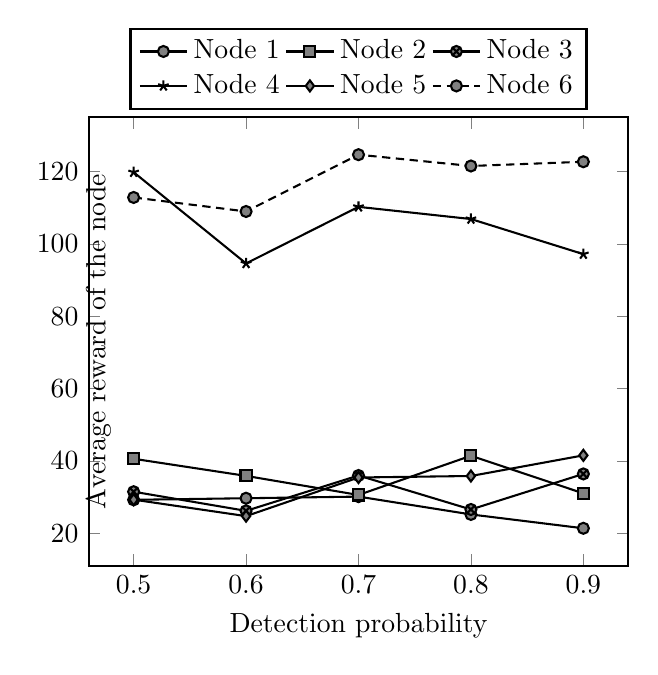
\begin{tikzpicture}
\begin{axis}[
  xlabel={Detection probability},
  ylabel={Average reward of the node },
  y label style={at={(0.06,0.5)}},
  xtick={0.5,0.6,0.7,0.8,0.9,1.0},
  legend style={at={(0.5,1.2)},cells={align=right}, anchor=north,legend columns=3},
  cycle list name=black white,
  grid style=dashed,
]

\addplot+[]
    coordinates {
(0.5,29.2207587022)(0.6,29.6591500811)(0.7,30.107769581)(0.8,25.1808225374)(0.9,21.3501334315)
};

\addplot+[]
    coordinates {
(0.5,40.5649596864)(0.6,35.8317201966)(0.7,30.5615817425)(0.8,41.4017616625)(0.9,31.0018428294)
};

\addplot+[]
    coordinates {
(0.5,31.4601711216)(0.6,26.1715912622)(0.7,35.9427616495)(0.8,26.5488358659)(0.9,36.3780765072)
};

\addplot+[]
    coordinates {
(0.5,119.788927983)(0.6,94.566243579)(0.7,110.212449824)(0.8,106.844518821)(0.9,97.138069126)
};

\addplot+[]
    coordinates {
(0.5,29.2697135288)(0.6,24.7098561839)(0.7,35.3909999115)(0.8,35.8083893589)(0.9,41.5087141375)
};

\addplot+[]
    coordinates {
(0.5,112.808511307)(0.6,108.932780706)(0.7,124.631408718)(0.8,121.507931814)(0.9,122.678991306)
};

\legend{Node 1, Node 2, Node 3, Node 4, Node 5, Node 6}
\end{axis}
\end{tikzpicture}

\caption{Nodes impact - Scenario a)}
\label{fig:nodeimp_single}
\end{figure}
\begin{figure}[h]
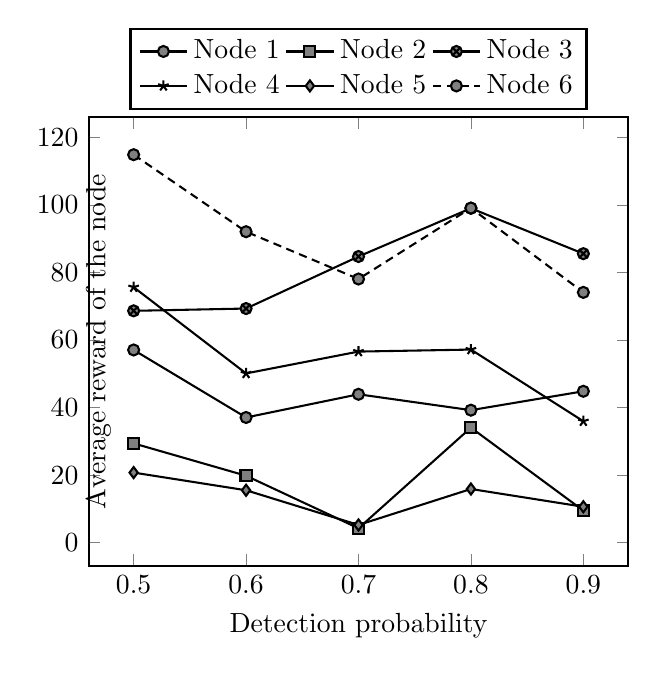
\begin{tikzpicture}
\begin{axis}[
  xlabel={Detection probability},
  ylabel={Average reward of the node },
  y label style={at={(0.06,0.5)}},
  xtick={0.5,0.6,0.7,0.8,0.9,1.0},
  legend style={at={(0.5,1.2)},cells={align=right}, anchor=north,legend columns=3},
  cycle list name=black white,
  grid style=dashed,
]

\addplot+[]
    coordinates {
(0.5,57.0711574474)(0.6,37.0782125822)(0.7,43.9471043804)(0.8,39.2446371458)(0.9,44.8363801675)
};

\addplot+[]
    coordinates {
(0.5,29.4097815394)(0.6,19.8278112984)(0.7,4.26428571429)(0.8,34.0706693208)(0.9,9.49928571429)
};

\addplot+[]
    coordinates {
(0.5,68.6596096998)(0.6,69.339332514)(0.7,84.7438538657)(0.8,99.0264041517)(0.9,85.5894326243)
};

\addplot+[]
    coordinates {
(0.5,75.6609039908)(0.6,50.1243516403)(0.7,56.5923700845)(0.8,57.1874277411)(0.9,35.9649500717)
};

\addplot+[]
    coordinates {
(0.5,20.7573450249)(0.6,15.5267400966)(0.7,5.25375523139)(0.8,15.8992854434)(0.9,10.6415647894)
};

\addplot+[]
    coordinates {
(0.5,114.89762846)(0.6,92.0949728442)(0.7,78.0795310037)(0.8,99.102629324)(0.9,74.1266846482)
};

\legend{Node 1, Node 2, Node 3, Node 4, Node 5, Node 6}
\end{axis}
\end{tikzpicture}
\caption{Nodes impact - Scenario b)}
\label{fig:nodeimp_multiple}
\end{figure}

\paragraph{Numerical results}
We have run the MDP using different budgets and detection probabilities.
Nodes are migrated in the following order: 1, 2 and 3.
The ordering of the nodes impacts the result sets of Algorithm~\ref{algo:target}, thus which nodes may be attacked at each transition.
We have extracted the monitoring set of each absorbing state, and evaluated the overall reward of each monitoring set.
We define the reward of a monitoring set as the weighted mean of the reward of each corresponding absorbing state.
The weighted mean uses the stationary distribution of the Markov Chain corresponding to the optimal policy.
The results are shown in Fig.~\ref{fig:nodeimp_single} for scenario a) and in Fig.~\ref{fig:nodeimp_multiple} for scenario b).

Based on the paths taken by attacks and the ordering of the migration, we can categorize the nodes into three categories: source, intermediate and border nodes.
The scenario a) sets the source to node 6, nodes 4 and 5 as intermediate nodes and finally nodes 1,2 and 3 as border nodes.
The scenario b) sets the source to nodes 3 and 6, nodes 1,4 as intermediate and nodes 2 and 5 as border nodes.
The first observation is that node 6 is globally the most rewarding node in both cases.
This is explained as it is the source of most of the attacks, and the exfiltrated data is redirected there.
In both scenarios the importance of nodes is separated according to the our categorization. 
This implies that the more the nodes will be on the path of attacks the more they get rewarded.
This is observation is reinforced in scenario b) where nodes 4 and 5 are close to attack sources while nodes 1 and 2 are further away.

In both scenarios, the detection rate does not have a significant impact on the ranking of the nodes, compared to each other.
The main trend in scenario a) is from $p=0.6$  node 4 does not overcome node 6 in reward. All other nodes remain closely grouped, and no intermediate or border nodes is standing out.
In scenario b) the higher the detection rate the higher the reward of node 3, the secondary source of attacks.
The steadiness in the evolution of each node shows that the performance of the detection is not a major factor in determining which nodes are best suited for the monitoring. We formulate some hypotheses in Section~\ref{sec:discussion}.
% For the single attack source, the importance of nodes compared to each other remains approximately constant, which implies that globally the performance in detecting attacks does not impact much where the resources should be deployed.
% We will show that specific exceptions may arise in Section~\ref{sec:apriori}.
% For multiple sources we observe that the detection rate has a bigger impact on which node is prioritized.
% When the detection rate is low, the system tends to prefer intermediate nodes, and even node 3, the source of some attacks does not rank better (at $p=0.5$).

Detailed examination of the optimal policy for each budget also shows that the action $m_j$ is never used to redeploy resource elsewhere in the infrastructure.
Instead of unmonitoring nodes, the MDP chooses the action $d$  to preserve the global detection probability.
$m_j$ actions are only chosen when the unmonitored node does not detect the next attack, thus having the same impact as action $d$. These corner cases only represent a small percentage of the global solution where very few attacks occurred.


\begin{table}[]
\begin{tabular}{|c|c|l|c|c|c|}
\hline
$b_f$   & \multicolumn{2}{c|}{$b_c$}         & p                     & $c_a$ & $\gamma$ \\ \hline
[30,40] & \multicolumn{2}{c|}{[10,20,30,40]} & [0.5,0.6,0.7,0.8,0.9] & 10    & 0.9      \\ \hline
\multicolumn{6}{|c|}{\{$V_1,V_2,V_3,V_4,V_5,V_6$\}}                                     \\ \hline
\multicolumn{6}{|c|}{[10,10,10,5,5,5]}                                                  \\ \hline
\end{tabular}
\caption{Parameters summary}
\label{tab:parameters}
\end{table}

\paragraph{A priori deployment}
\label{sec:apriori}
When solving a problem using an MDP, the solution is a dynamic proposition to choose actions as the system evolves.
However, from a technical aspect, the defender needs to have the nodes already monitoring the infrastructure before starting the migration process.
It becomes necessary to translate the dynamic answer of the MDP into a static \textit{a priori} deployment.
After determining the individual importance of each node, we propose to determine the optimal set of monitoring nodes.

The main difference is that each node was evaluated based on all the possible budget combinations, whereas what is defined here is a particular answer for a specific budget.
For each budget, the maximum reward is $\frac{b_f}{c_a} \sum\limits_{i \in \textbf{N}}V_i $ which corresponds to the corner case where the attacker never launched an attack, and we can evaluate the efficiency of the   monitoring nodes thanks to the associated reward.
Even if a particular monitoring set achieves close to the maximum reward, it is also because the set is tailored to a subset of all possible attacks.
We propose to determine the optimal monitoring state for each budget by weighting the reward they achieve with their occupation of the total solution space.

We note $S_{\text{abs}}$ the set of absorbing states, $S^{\text{Mo}}_{\text{abs}}$ the set of absorbing states with a common  monitoring set $Mo$, $\rho(Mo)$ the percentage of presence of set $Mo$ in the solution space and $R(Mo)$ the reward of monitoring set $Mo$.
% \begin{equation}
%     R(Mo) = \sum\limits_{s \in S_{Mo}^{abs}}\rho(Mo^s)R(Mo^s)
% \end{equation}
Then we propose to choose the optimal monitoring set $Mo^*$ with:
\begin{equation}
    Mo^* = \argmax\limits_{\text{Mo} \in S_{\text{abs}}} \left \{\sum\limits_{s \in S^{\text{Mo}}_{\text{abs}}}\rho(Mo^s)R(Mo^s) \right \}
\end{equation}

We present the results for scenario a) in Table~\ref{tab:optiset}.
We observe that nodes 4 and 6 are always chosen in the monitoring, which corresponds to Fig.~\ref{fig:nodeimp_single}.
Node 1 also often appears as a good candidate for a fourth node if it is not already chosen third.
With $p=0.7$ we observe that third and fourth nodes do not coincidate between (30,30) and (40,40) budgets.
This suggests that the combining two nodes increases their individual performance.
(Node 1 is surrounded by node 2 and 3 in the topology).
% This is explained because other budgets impact the individual importance of each node.

% Please add the following required packages to your document preamble:
% \usepackage{multirow}
% \usepackage{graphicx}
\begin{table}[h]
\resizebox{\textwidth}{!}{%
\begin{tabular}{ccccccc}
\multicolumn{3}{c}{\textbf{Scenario a)}}                                                                     &                       & \multicolumn{3}{c}{\textbf{Scenario b)}}                                                                    \\ \cline{1-3} \cline{5-7} 
\multicolumn{1}{|c|}{p}                    & \multicolumn{1}{c|}{($b_f,b_c$)} & \multicolumn{1}{c|}{$Mo^*$}  & \multicolumn{1}{c|}{} & \multicolumn{1}{c|}{p}                    & \multicolumn{1}{c|}{($b_f,b_c$)} & \multicolumn{1}{c|}{$Mo^*$}  \\ \cline{1-3} \cline{5-7} 
\multicolumn{1}{|c|}{\multirow{2}{*}{0.5}} & \multicolumn{1}{c|}{(30,30)}     & \multicolumn{1}{c|}{2,4,6}   & \multicolumn{1}{c|}{} & \multicolumn{1}{c|}{\multirow{2}{*}{0.5}} & \multicolumn{1}{c|}{(30,30)}     & \multicolumn{1}{c|}{2,4,6}   \\ \cline{2-3} \cline{6-7} 
\multicolumn{1}{|c|}{}                     & \multicolumn{1}{c|}{(40,40)}     & \multicolumn{1}{c|}{1,2,4,6} & \multicolumn{1}{c|}{} & \multicolumn{1}{c|}{}                     & \multicolumn{1}{c|}{(40,40)}     & \multicolumn{1}{c|}{1,2,4,6} \\ \cline{1-3} \cline{5-7} 
\multicolumn{1}{|c|}{\multirow{2}{*}{0.7}} & \multicolumn{1}{c|}{(30,30)}     & \multicolumn{1}{c|}{1,4,6}   & \multicolumn{1}{c|}{} & \multicolumn{1}{c|}{\multirow{2}{*}{0.7}} & \multicolumn{1}{c|}{(30,30)}     & \multicolumn{1}{c|}{1,4,6}   \\ \cline{2-3} \cline{6-7} 
\multicolumn{1}{|c|}{}                     & \multicolumn{1}{c|}{(40,40)}     & \multicolumn{1}{c|}{2,3,4,6} & \multicolumn{1}{c|}{} & \multicolumn{1}{c|}{}                     & \multicolumn{1}{c|}{(40,40)}     & \multicolumn{1}{c|}{2,3,4,6} \\ \cline{1-3} \cline{5-7} 
\multicolumn{1}{|c|}{\multirow{2}{*}{0.9}} & \multicolumn{1}{c|}{(30,30)}     & \multicolumn{1}{c|}{4,5,6}   & \multicolumn{1}{c|}{} & \multicolumn{1}{c|}{\multirow{2}{*}{0.9}} & \multicolumn{1}{c|}{(30,30)}     & \multicolumn{1}{c|}{4,5,6}   \\ \cline{2-3} \cline{6-7} 
\multicolumn{1}{|c|}{}                     & \multicolumn{1}{c|}{(40,40)}     & \multicolumn{1}{c|}{1,4,5,6} & \multicolumn{1}{c|}{} & \multicolumn{1}{c|}{}                     & \multicolumn{1}{c|}{(40,40)}     & \multicolumn{1}{c|}{1,4,5,6} \\ \cline{1-3} \cline{5-7} 
                                           &                                  &                              &                       &                                           &                                  &                              \\
\multicolumn{3}{c}{\textbf{Scenario c)}}                                                                     &                       & \multicolumn{3}{c}{\textbf{Scenario d)}}                                                                    \\ \cline{1-3} \cline{5-7} 
\multicolumn{1}{|c|}{p}                    & \multicolumn{1}{c|}{($b_f,b_c$)} & \multicolumn{1}{c|}{$Mo^*$}  & \multicolumn{1}{c|}{} & \multicolumn{1}{c|}{p}                    & \multicolumn{1}{c|}{($b_f,b_c$)} & \multicolumn{1}{c|}{$Mo^*$}  \\ \cline{1-3} \cline{5-7} 
\multicolumn{1}{|c|}{\multirow{2}{*}{0.5}} & \multicolumn{1}{c|}{(30,30)}     & \multicolumn{1}{c|}{1,2,6}   & \multicolumn{1}{c|}{} & \multicolumn{1}{c|}{\multirow{2}{*}{0.5}} & \multicolumn{1}{c|}{(30,30)}     & \multicolumn{1}{c|}{1,3,6}   \\ \cline{2-3} \cline{6-7} 
\multicolumn{1}{|c|}{}                     & \multicolumn{1}{c|}{(40,40)}     & \multicolumn{1}{c|}{1,3}     & \multicolumn{1}{c|}{} & \multicolumn{1}{c|}{}                     & \multicolumn{1}{c|}{(40,40)}     & \multicolumn{1}{c|}{1,2,3,6} \\ \cline{1-3} \cline{5-7} 
\multicolumn{1}{|c|}{\multirow{2}{*}{0.7}} & \multicolumn{1}{c|}{(30,30)}     & \multicolumn{1}{c|}{1,3,6}   & \multicolumn{1}{c|}{} & \multicolumn{1}{c|}{\multirow{2}{*}{0.7}} & \multicolumn{1}{c|}{(30,30)}     & \multicolumn{1}{c|}{1,2,6}   \\ \cline{2-3} \cline{6-7} 
\multicolumn{1}{|c|}{}                     & \multicolumn{1}{c|}{(40,40)}     & \multicolumn{1}{c|}{1,2,3,6} & \multicolumn{1}{c|}{} & \multicolumn{1}{c|}{}                     & \multicolumn{1}{c|}{(40,40)}     & \multicolumn{1}{c|}{1,2,5,6} \\ \cline{1-3} \cline{5-7} 
\multicolumn{1}{|c|}{\multirow{2}{*}{0.9}} & \multicolumn{1}{c|}{(30,30)}     & \multicolumn{1}{c|}{1,3,6}   & \multicolumn{1}{c|}{} & \multicolumn{1}{c|}{\multirow{2}{*}{0.9}} & \multicolumn{1}{c|}{(30,30)}     & \multicolumn{1}{c|}{1,2,6}   \\ \cline{2-3} \cline{6-7} 
\multicolumn{1}{|c|}{}                     & \multicolumn{1}{c|}{(40,40)}     & \multicolumn{1}{c|}{1,2,3,6} & \multicolumn{1}{c|}{} & \multicolumn{1}{c|}{}                     & \multicolumn{1}{c|}{(40,40)}     & \multicolumn{1}{c|}{1,2,3,6} \\ \cline{1-3} \cline{5-7} 
                                           &                                  &                              &                       &                                           &                                  &                              \\
\multicolumn{3}{c}{\textbf{Scenario e)}}                                                                     &                       & \multicolumn{3}{c}{\textbf{Scenario f)}}                                                                    \\ \cline{1-3} \cline{5-7} 
\multicolumn{1}{|c|}{p}                    & \multicolumn{1}{c|}{($b_f,b_c$)} & \multicolumn{1}{c|}{$Mo^*$}  & \multicolumn{1}{c|}{} & \multicolumn{1}{c|}{p}                    & \multicolumn{1}{c|}{($b_f,b_c$)} & \multicolumn{1}{c|}{$Mo^*$}  \\ \cline{1-3} \cline{5-7} 
\multicolumn{1}{|c|}{\multirow{2}{*}{0.5}} & \multicolumn{1}{c|}{(30,30)}     & \multicolumn{1}{c|}{2,3,6}   & \multicolumn{1}{c|}{} & \multicolumn{1}{c|}{\multirow{2}{*}{0.5}} & \multicolumn{1}{c|}{(30,30)}     & \multicolumn{1}{c|}{1,2,6}   \\ \cline{2-3} \cline{6-7} 
\multicolumn{1}{|c|}{}                     & \multicolumn{1}{c|}{(40,40)}     & \multicolumn{1}{c|}{1,2,3,6} & \multicolumn{1}{c|}{} & \multicolumn{1}{c|}{}                     & \multicolumn{1}{c|}{(40,40)}     & \multicolumn{1}{c|}{1,2,3,6} \\ \cline{1-3} \cline{5-7} 
\multicolumn{1}{|c|}{\multirow{2}{*}{0.7}} & \multicolumn{1}{c|}{(30,30)}     & \multicolumn{1}{c|}{2,3,6}   & \multicolumn{1}{c|}{} & \multicolumn{1}{c|}{\multirow{2}{*}{0.7}} & \multicolumn{1}{c|}{(30,30)}     & \multicolumn{1}{c|}{1,2,6}   \\ \cline{2-3} \cline{6-7} 
\multicolumn{1}{|c|}{}                     & \multicolumn{1}{c|}{(40,40)}     & \multicolumn{1}{c|}{2,6}     & \multicolumn{1}{c|}{} & \multicolumn{1}{c|}{}                     & \multicolumn{1}{c|}{(40,40)}     & \multicolumn{1}{c|}{1,2,3,6} \\ \cline{1-3} \cline{5-7} 
\multicolumn{1}{|c|}{\multirow{2}{*}{0.9}} & \multicolumn{1}{c|}{(30,30)}     & \multicolumn{1}{c|}{2,3,6}   & \multicolumn{1}{c|}{} & \multicolumn{1}{c|}{\multirow{2}{*}{0.9}} & \multicolumn{1}{c|}{(30,30)}     & \multicolumn{1}{c|}{1,2,6}   \\ \cline{2-3} \cline{6-7} 
\multicolumn{1}{|c|}{}                     & \multicolumn{1}{c|}{(40,40)}     & \multicolumn{1}{c|}{2,3,5,6} & \multicolumn{1}{c|}{} & \multicolumn{1}{c|}{}                     & \multicolumn{1}{c|}{(40,40)}     & \multicolumn{1}{c|}{1,2,4,6} \\ \cline{1-3} \cline{5-7} 
\end{tabular}%
}
\caption{Optimal monitoring sets of the use cases}
\label{tab:mdp-usecase-optiset}
\end{table}

\subsubsection{Discussion}
\label{sec:discussion}
In this section, we propose to discuss some of the limitations and findings of our approach.
The main limitation of the model is the size of the numerical use case. Since the MDP set of states and transitions are generated recursively, the bigger the topology and the budgets the bigger the computation time.
Because of the use of the $m_j$ action as an equivalent to action $d$, we assume that the relocation of monitoring resources would happen in bigger use cases, but those cannot be generated due to combinatory explosion.

In Section~\ref{sec:apriori} we proposed a method to determine for each budget what was the optimal monitoring set.
This method supposes that the ordering of the monitoring deployment does not impact the rewards obtained.
While this is not true when considering individually each path from the starting state to an absorbing state, the aggregation of the results toward monitoring sets reduces the impact of this assumption.
In addition to that, we have defined an attacker model in which the target decision is not based on which security measures are already deployed on the infrastructure, thus making the target decision space independent from the monitoring.
% Obviously, each monitoring decision will have a different impact for the defender depending on which node is being attacked for the next transition, but this does not affect the attacker.

We have observed the importance of the detection probability in our use case and concluded that it was not an impacting parameter in determining the optimal monitoring set.
However, topologies where important nodes could be reached from several paths and where there could be multiple data exfiltration paths could lead to choosing intermediate nodes over border nodes.